\documentclass[t]{beamer}
\usetheme{Warsaw}
\usecolortheme{seahorse}
\usepackage{array}
\usepackage{graphicx}
\usepackage{amssymb,amsmath,mathrsfs,amsfonts}
%\usepackage[colorhighlight,display]{texpower}
%\usepackage{caption}
%\usepackage[all]{xy}
\usepackage{beamerthemesplit}
\mode<presentation>
%\usepackage{pause}
\usepackage{ulem}  % for strikethroughs
\usepackage{cancel} % for strikethroughs in math mode 
\usepackage{tikz}
\usepackage{calc}
\usetikzlibrary{shapes}
\usepackage{hyperref}
\hypersetup{pdfpagemode=FullScreen}
\usepackage{ifthen}
\usepackage{animate}
\usepackage{color}
\usepackage{type1cm}  % used for watermarking
\usepackage{eso-pic}  % used for watermarking
\usepackage[absolute,overlay]{textpos}
  \setlength{\TPHorizModule}{1mm}
  \setlength{\TPVertModule}{1mm}


\theoremstyle{plain}
\newtheorem{prop}{Proposition}
\newtheorem{thm}[prop]{Theorem}
\newtheorem{lem}[prop]{Lemma}
\newtheorem{cor}[prop]{Corollary}
\theoremstyle{definition}
\newtheorem{dfn}{Definition}
\newtheorem{rem}[prop]{Remark}
\newtheorem{ex}{Example}[section]
%\newtheorem{note}{Note}[section]
\newtheorem{exercise}{Exercise}[section]
\newcommand{\nin}{\noindent}
\newcommand{\ds}{\displaystyle}
\renewcommand{\figurename}{Figure \arabic{figure}}
\renewcommand*\familydefault{\sfdefault} 


%%%%%%%%%%%%%%%%%%%%%%%%%%5
%%%%%%%%%%%%%%%%%%%%%%%%%%%%
%%%% some commands that have different meaning in the article/presentation modes

\newcommand{\vvfill}{\mode<presentation>{\vfill}  \mode<article>{\medskip}}   %vfill in presentation only
\newcommand{\sketchspace}{ 
\mode<article>{ \medskip\noindent{\textbf{Sketch:}} \vspace*{6cm} }
\mode<presentation>{ } 
}
\newcommand{\examplespace}{ 
\mode<article>{ \medskip\noindent{\textbf{Example:}} \vspace{6cm} }
\mode<presentation>{ } 
}
\newcommand{\artsmspace}{\mode<article>{\vspace*{2cm}} }  %small space in article mode
\newcommand{\artlargespace}{\mode<article>{\vspace*{6cm}} }  %large space in article mode

\newcommand{\dx}{\,dx}

\newcommand{\soln}{{\textbf{Solution: }}\,\,\,}
\newcommand{\disp}{\displaystyle}

\newcommand{\makedate}{\vvfill
\begin{picture}(10,10)  
\put(260,-20){\mbox{\tiny{\today}}}
\end{picture}
}

\newcommand{\pd}[2]{\dfrac{\partial#1}{\partial#2}}
\newcommand{\pD}[2]{\dfrac{\partial^2#1}{\partial#2^2}}
\newcommand{\pdd}[3]{\dfrac{\partial^2#1}{\partial#2 \partial#3}}


\normalem %stops the ulem package making all the emphs into underlines...
 
 
 
 \newcommand{\refandrev}[2]{
 \begin{small}
  \hspace{6cm}
  \begin{minipage}[r]{8cm}
  Stewart,    Chapter #1   \\
  Review:  \parbox[t]{6cm}{#2}
\end{minipage}
\end{small}
}



\newcounter{heading}
\setcounter{section}{1}
\setcounter{heading}{0}

\newcommand{\makeheading}[1]{\medskip\begin{large}\noindent\textbf{{#1}}\end{large}\smallskip}

%\newenvironment{head}[1]{\medskip\stepcounter{heading}\noindent\textbf{\hspace{0.2cm}{#1}.}}{}
\newcommand{\newhead}[1]{\medskip\stepcounter{heading}\noindent\textbf{\hspace{0.2cm}{#1}.}}


\newcommand{\pf}[1]{\noindent\textit{Proof.}\vspace*{#1 cm}}
\newcommand{\sol}[1]{\noindent\textit{Solution.}\vspace*{#1 cm}}
\newcommand{\further}[1]{\begin{small}\noindent\textit{Further reading: #1}\end{small}}
\newcommand{\exr}[1]{\begin{footnotesize}\noindent\textit{\textbf{Exercises:} Stewart #1}\end{footnotesize}}


% Sets of numbers
\newcommand{\C}{\mathbb{C}}
\newcommand{\RR}{\mathbb{R}}
\newcommand{\Z}{\mathbb{Z}}
\newcommand{\N}{\mathbb{N}}
\newcommand{\Q}{\mathbb{Q}}

% Partitions
\newcommand{\PP}{\mathcal{P}}

% Limits
\newcommand{\limm}[1]{\displaystyle \lim_{x\to #1}}

% Backslash
\newcommand{\bs}{\backslash}

% functions
\newcommand{\cosec}{\mathrm{cosec}}
\newcommand{\cosech}{\mathrm{cosech}}
\newcommand{\sech}{\mathrm{sech}}
\newcommand{\Li}{\mathrm{Li}}
\newcommand{\si}{\mathrm{Si}}
\newcommand{\erf}{\mathrm{erf}}

% Domain and Range
\newcommand{\Dom}{\mathrm{Dom}}
\newcommand{\Codom}{\mathrm{Codom}}
\newcommand{\Range}{\mathrm{Ran}}



\title{Week 11:  Integration Techniques Part 3}

\begin{document}

\frame{\titlepage}

\setcounter{tocdepth}{2}
\frame{\tableofcontents

}

\AtBeginSection[]
{
\begin{frame}<beamer> 
\tableofcontents[currentsection]  % show TOC and highlight current section
\end{frame}
}

\section{Integration of Rational Functions by Partial Functions - Part 1 }

\begin{frame}
\frametitle{Integrating rational functions}

In this section we show how to integrate any rational function (a ratio of polynomials) by expressing it as a sum of simpler fractions, called \textit{partial fractions}, that we already know how to integrate. To illustrate the method, observe that:

$$\frac{2}{x-1} - \frac{1}{x+2} = \frac{2(x+2)-(x-1)}{(x-1)(x+2)} = \frac{x + 5}{x^2 + x - 2}$$

If we now reverse the procedure, we see how to integrate the fnction:

\begin{align*}
\displaystyle\int\frac{x+5}{x^2 + x - 2}dx &= \int\left(\frac{2}{x-1} - \frac{1}{x+2}\right)dx\\
&= 2 \ln|x - 1| - \ln|x + 2| + C
\end{align*}


\end{frame}

\begin{frame}
\frametitle{Example}

Find $\displaystyle\int\frac{x^3 + x}{x - 1}$ \pause

\begin{align*}
\displaystyle\frac{x^3 + x}{x - 1}dx &= \int\left(x^2 + x + 2 + \frac{2}{x-1}\right)dx\\
&= \frac{x^3}{3} + \frac{x^2}{2} + 2x + 2 \ln |x - 1| + C
\end{align*}

\begin{textblock}{0.3}(100,0)
      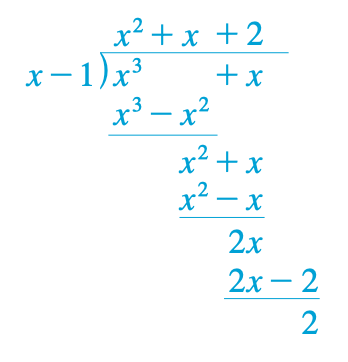
\includegraphics[scale=0.45]{fig/divide}
\end{textblock}

\end{frame}

\begin{frame}
\noindent\underline{\textit{Case 1:} The denominator splits into distinct linear factors.}
Examples of two such rational functions and the form of their partial fractions decompositions are given below:
\begin{align*}
\frac{x-3}{(x-1)(x-2)}&= {\frac{A}{x-1}+\frac{B}{x-2}}\\
\frac{x^2-x+7}{x(2x+1)(x-3)}&= {\frac{A}{x}+\frac{B}{2x+1}+\frac{C}{x-3}}.
\end{align*}

\end{frame}

\begin{frame}
\footnotesize
\frametitle{Example}

Evaluate $\displaystyle\int\frac{x^2 + 2x - 1}{2x^3 + 3x^2 - 2x}dx$ \pause

\medskip

Since the degree of the numerator (top one) is less than the degree of the denominator, we don't divide.  Instead, we factor the denominator as

$$2x^3 + 3x^2 - 2x = x(2x^2 + 3x - 2) = x(2x - 1)(x + 2)$$

We can do the partial fraction as:

$$\frac{x^2 + 2x - 1}{x(2x - 1)(x + 2)} = \frac{A}{x} + \frac{B}{2x - 1} + \frac{C}{x + 2}$$

To find A, B, C, we multiply both sides:

$$x^2 + 2x - 1 = A(2x - 1)(x + 2) + Bx(x + 2) + Cx(2x - 1)$$

We can rewrite as:

$$x^2 + 2x - 1 = (2A + B + 2C)x^2 + (3A + 2B - C)x - 2A$$

\textit{(continued next slide)}

\end{frame}

\begin{frame}
\footnotesize

\newhead{continued...}

Coefficients on both sides of the equation must be equal, thus:

\begin{align*}
2A + B + 2C &= 1\\
3A + 2B - C &= 2\\
-2A &= -1
\end{align*}

Solving this, we get $A = \frac{1}{2}$, $B = \frac{1}{5}$, $C = -\frac{1}{10}$, and so

\begin{align*}
\int\frac{x^2 + 2x - 1}{2x^3 + 3x^2 - 2x}dx &= \int\left(\frac{1}{2}\frac{1}{x} + \frac{1}{5}\frac{1}{2x - 1} - \frac{1}{10}\frac{1}{x + 2}\right)dx\\
&= \frac{1}{2}\ln|x| + \frac{1}{10}\ln|2x - 1| - \frac{1}{10}\ln|x + 2| + C
\end{align*}

Note that when we integrate the middle term, we made the substitution $u = 2x - 1$ which gives $du = 2dx$, and $dx = \frac{1}{2}du$

\end{frame}



\begin{frame}
\noindent\underline{\textit{Case 2:} The denominator has a repeated linear factor.}\\
Examples of two such rational functions and the form of their partial fractions decompositions are given below:
\begin{align*}
\frac{x^2+1}{(x+4)^3}&= {\frac{A}{x+4}+\frac{B}{(x+4)^2}+\frac{C}{(x+4)^3}}\\
\frac{x^2-2}{(x-1)(x-2)^2}&= {\frac{A}{x-1}+\frac{B}{x-2}+\frac{C}{(x-2)^2}}.
\end{align*}
\end{frame}

\begin{frame}
\footnotesize
\frametitle{Example}
Find $\displaystyle\int \frac{x^4 - 2x^2 + 4x + 1}{x^3 - x^2 - x + 1}dx$ \pause

\medskip

The first step is to divide.  The result of long division is

$$ \frac{x^4 - 2x^2 + 4x + 1}{x^3 - x^2 - x + 1} = x + 1 + \frac{4x}{x^3 - x^2 - x + 1}$$

The second step is to factor the denominator.  Since $Q(1) = 0$, we know that $x - 1$ is a factor and we obtain:

$$x^3 - x^2 - x + 1 = (x - 1)(x^2 - 1) = (x - 1)(x-1)(x+1) = (x-1)^2(x+1)$$

Since the linear factor $x-1$ occurs twice, the partial fraction decomposition is

$$\frac{4x}{(x-1)^2(x+1)} = \frac{A}{x-1} + \frac{B}{(x-1)^2} + \frac{C}{x + 1}$$

\textit{(continued next slide)}

\end{frame}

\begin{frame}
\footnotesize
\newhead{Continued...}

Multiplying by the least common denominator, $(x-1)^2(x+1)$, we get

$$4x = A(x-1)(x+1) + B(x + 1) + C(x-1)^2$$

Equating coefficients, we get:

\begin{align*}
A + C &= 0\\
B - 2C &= 4\\
-A + B + C &= 0\\
\end{align*}

Solving this, we get $A = 1, B = 2, C = -1$, so

\begin{align*}
\displaystyle\int \frac{x^4 - 2x^2 + 4x + 1}{x^3 - x^2 - x + 1}dx &= \int\left[x + 1 + \frac{1}{x-1} + \frac{2}{(x-1)^2} - \frac{1}{x + 1}\right]dx\\
&= \frac{x^2}{2} + x + \ln|x - 1| - \frac{2}{x-1} - \ln|x + 1| + C\\
&= \frac{x^2}{2} + x - \frac{2}{x - 1} + \ln\left|\frac{x - 1}{x + 1}\right| + C
\end{align*}

\end{frame}

\begin{frame}
\frametitle{Exercise}

\begin{itemize}
	\item $\displaystyle\int\frac{5x + 1}{(2x + 1)(x-1)}dx$ %Stewart chapter 7.4 No. 9
	\begin{itemize}
		\item Ans: $\frac{1}{2}\ln|2x + 1| + 2 \ln|x - 1| + C$
	\end{itemize}
	\item  $\displaystyle\int \frac{x^4 - 2x^2 + 4x + 1}{x^3 - x^2 - x + 1}dx$ %Stewart chapter 7.4. Example4
	\begin{itemize}
		\item Ans: $\frac{x^2}{2} + x - \frac{2}{x - 1} + \ln{|\frac{x - 1}{x + 1}|} + C$
	\end{itemize}
	\item$\displaystyle\int\frac{dx}{x^2 - a^2}$  %Stewart chapter 7.4. Example3
	\begin{itemize}
		\item Ans: $\frac{1}{2a}\ln{\left|\frac{x - a}{x + a}\right|} + C$
	\end{itemize}
	\item $\displaystyle\int\frac{x^3 + 4x^2 + x - 1}{x^3 + x^2}dx$ %Stewart chapter 7.4 No. 16
	\begin{itemize}
		\item Ans: $\frac{1}{2} + \ln 6$
	\end{itemize}
\end{itemize}

\end{frame}

\section{Integration of Rational Functions by Partial Functions - Part 2}


\begin{frame}
\noindent\underline{\textit{Case 3:} The denominator has an irreducible quadratic factor.}
Examples of two such rational functions and the form of their partial fractions decomposition are given below:
\begin{align*}
\frac{x^2+x}{(x-1)(x^2+9)}&= {\frac{A}{x-1}+\frac{Bx+C}{x^2+9}}\\
\frac{x^3-2x+4}{(x^2+5)(x^2+x+1)}&= {\frac{Ax+B}{x^2+5}+\frac{Cx+D}{x^2+x+1}}.
\end{align*}

Note that irreducible quadratic factor of $ax^2 + bx + c$ has determinants of $b^2 - 4ac < 0$

\end{frame}

\begin{frame}
\footnotesize
\frametitle{Example}
Find $\displaystyle\int\frac{2x^2 - x + 4}{x^3 + 4x}dx$

Since $x^3 + 4x = x(x^2 + 4)$ can't be factored further, we write

$$\frac{2x^2 - x + 4}{x(x^2 + 4)} = \frac{A}{x} + \frac{Bx + C}{x^2 + 4}$$

Multiplying both sides:

\begin{align*}
2x^2 - x + 4 &= A(x^2 + 4) + (Bx + C)x\\
&= (A + B)x^2 + Cx + 4A
\end{align*}

Equating coefficients:

$$A + B = 2 \qquad C = -1 \qquad 4A = 4$$

Thus $A = 1, B = 1, C = -1$,   \textit{(continued next slide)}

\end{frame}

\begin{frame}
\footnotesize
\newhead{Continued...}

\begin{align*}
\displaystyle\int\frac{2x^2 - x + 4}{x^3 + 4x}dx &= \int \frac{1}{x} + \left(\frac{x - 1}{x^2 + 4}\right)dx \\
&= \int\frac{1}{x}dx + \int\frac{x}{x^2 + 4} - \int\frac{1}{x^2 + 4}dx\\
&=\ln |x|+ \frac{1}{2}\ln(x^2 + 4) - \frac{1}{2}\tan^{-1}(\frac{x}{2}) + C
\end{align*}

Note that in the second step, we let $u = x^2 + 4$ so $du = 2xdx$.  Also note that $\int\frac{1}{a^2+x^2}\,dx=\frac{1}{a}\tan^{-1}\frac{x}{a}+C$

\end{frame}

\begin{frame}
\noindent\underline{\textit{Case 4:} The denominator has a repeated irreducible quadratic factor.}
It has the form as follows:
\begin{align*}
\frac{x^2+x}{(x^2+9)^3}&= {\frac{Ax+B}{x^2+9}+\frac{Cx+D}{(x^2+9)^2}+\frac{Ex+F}{(x^2+9)^3}}\\
\frac{x^3-2x+4}{(x-2)(x^2+x+1)^2}&= {\frac{A}{x-2}+\frac{Bx+C}{x^2+x+1}+\frac{Dx+E}{(x^2+x+1)^2}}.
\end{align*}
\end{frame}

\begin{frame}
\footnotesize
\frametitle{Example}
Find $\displaystyle\int\frac{1 - x + 2x^2 - x^3}{x(x^2 + 1)^2}dx$\pause

\medskip

The form of the decomposition is

$$\displaystyle\int\frac{1 - x + 2x^2 - x^3}{x(x^2 + 1)^2} = \frac{A}{x} + \frac{Bx + C}{x^2 + 1} + \frac{Dx + E}{(x^2 + 1)^2}$$

Multiplying both sides:

\begin{align*}
-x^3 + 2x^2 - x + 1 &= A(x^2 + 1)^2 + (Bx + C)x(x^2 + 1) + (Dx + E)x\\
&= A(x^4 + 2x^2 + 1) + B(x^4 + x^2) + C(x^3 + x) + Dx^2 + Ex\\
&= (A + B)x^4 + Cx^3 + (2A + B + D)x^2 + (C + E)x + A
\end{align*}

Equating the coefficients, we get:

$$A + B = 0 \qquad C = -1 \qquad 2A + B + D = 2 \qquad C + E = -1 \qquad A = 1$$
$$ A =1, B = -1, C = -1, D = 1, E = 0$$

\textit{(continued next slide)}

\end{frame}

\begin{frame}
\footnotesize
\newhead{Continued...}

\begin{align*}
\displaystyle\int\frac{1 - x + 2x^2 - x^3}{x(x^2 + 1)^2}dx &= \int\left(\frac{1}{x} - \frac{x + 1}{x^2 + 1} + \frac{x}{(x^2 + 1)^2}\right)dx\\
&= \int\frac{dx}{x} - \int\frac{x}{x^2 + 1}dx - \int\frac{dx}{x^2 + 1} + \int\frac{xdx}{(x^2 + 1)^2}\\
&= \ln|x| - \frac{1}{2}\ln(x^2 + 1) - \tan^{-1}x - \frac{1}{2(x^2 + 1)} + C
\end{align*}

Note that we made a mental substitution of $u = x^2 + 1$ in second and fourth terms.

\end{frame}

\begin{frame}
\frametitle{Exercise}
\begin{itemize}
	\item  $\displaystyle\int\frac{x^2 - x + 6}{x^3 + 3x}dx$%Stewart chapter 7.4 No. 24
	\begin{itemize}
		\item Ans: $2\ln|x| - \frac{1}{2}\ln(x^2 + 3) - \frac{1}{\sqrt{3}}\tan^{-1}\frac{x}{\sqrt{3}} + C$
	\end{itemize}
	\item  $\displaystyle\int\frac{x^3 + 6x - 2}{x^4 + 6x^2}dx$%Stewart chapter 7.4 No. 28
	\begin{itemize}
		\item Ans: $\ln|x| + \frac{1}{3x} + \frac{1}{3\sqrt{6}}\tan^{-1}\left(\frac{x}{\sqrt{6}}\right) + C$
	\end{itemize}
\end{itemize}

\end{frame}


\end{document}